\begin{tikzpicture}[scale=1.4] 
\node (hidden0) at (0.0,3.0) {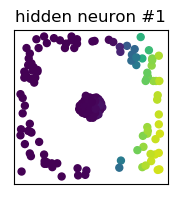
\includegraphics[width=1.6cm]{mfp/learning_process/h_neuron_500_1.png}}; 
\node (hidden1) at (1.0,3.0) {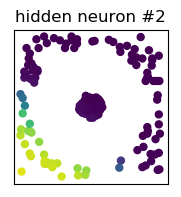
\includegraphics[width=1.6cm]{mfp/learning_process/h_neuron_500_2.png}}; 
\node (hidden2) at (2.0,3.0) {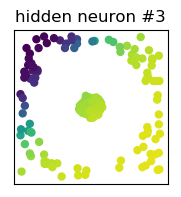
\includegraphics[width=1.6cm]{mfp/learning_process/h_neuron_500_3.png}}; 
\node (hidden3) at (3.0,3.0) {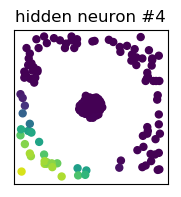
\includegraphics[width=1.6cm]{mfp/learning_process/h_neuron_500_4.png}}; 
\node (hidden4) at (4.0,3.0) {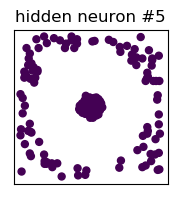
\includegraphics[width=1.6cm]{mfp/learning_process/h_neuron_500_5.png}}; 
\node (hidden5) at (5.0,3.0) {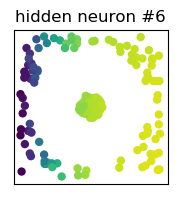
\includegraphics[width=1.6cm]{mfp/learning_process/h_neuron_500_6.png}}; 
\node (hidden6) at (6.0,3.0) {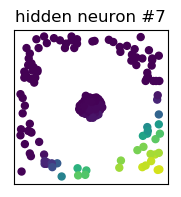
\includegraphics[width=1.6cm]{mfp/learning_process/h_neuron_500_7.png}}; 
\node (hidden7) at (7.0,3.0) {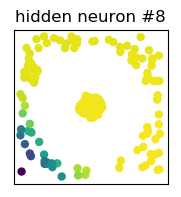
\includegraphics[width=1.6cm]{mfp/learning_process/h_neuron_500_8.png}}; 
\node (hidden8) at (8.0,3.0) {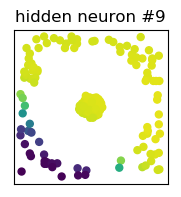
\includegraphics[width=1.6cm]{mfp/learning_process/h_neuron_500_9.png}}; 
\node (hidden9) at (9.0,3.0) {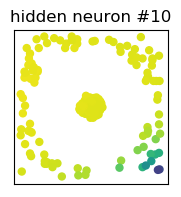
\includegraphics[width=1.6cm]{mfp/learning_process/h_neuron_500_10.png}}; 
\node (hidden10) at (10.0,3.0) {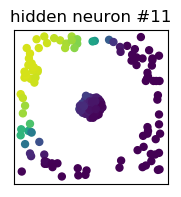
\includegraphics[width=1.6cm]{mfp/learning_process/h_neuron_500_11.png}}; 
\node (out500) at (5.2,.85) {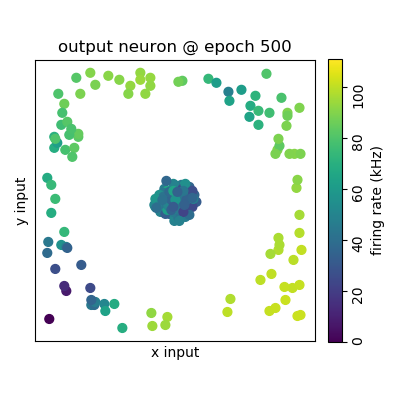
\includegraphics[width=3.6cm]{mfp/learning_process/output_neuron_500.png}}; 

\draw[-stealth,line width=1.5pt, color=red ] (hidden0.south) -- (out500); 
\draw[-stealth,line width=0.1pt, color=blue ] (hidden1.south) -- (out500); 
\draw[-stealth,line width=0.8pt, color=red ] (hidden2.south) -- (out500); 
\draw[-stealth,line width=0.7pt, color=red ] (hidden3.south) -- (out500); 
\draw[-stealth,line width=1.2pt, shorten >= -.5cm, color=red ] (hidden4.south) -- (out500); 
\draw[-stealth,line width=2.0pt, shorten >= -.4cm, color=red ] (hidden5.south) -- (out500); 
\draw[-stealth,line width=2.3pt, shorten >= -.5cm, color=red ] (hidden6.south) -- (out500); 
\draw[-stealth,line width=0.9pt, shorten >= -.4cm, color=red ] (hidden7.south) -- (out500); 
\draw[-stealth,line width=0.5pt, color=blue ] (hidden8.south) -- (out500); 
\draw[-stealth,line width=0.2pt, color=red ] (hidden9.south) -- (out500); 
\draw[-stealth,line width=2.2pt, color=red ] (hidden10.south) -- (out500); 
\end{tikzpicture} 